\documentclass[a4paper,12pt]{article} 

% First, we usually want to set the margins of our document. For this we use the package geometry.
\usepackage[top = 2.5cm, bottom = 2.5cm, left = 2.5cm, right = 2.5cm]{geometry} 
\usepackage[T1]{fontenc}
\usepackage[utf8]{inputenc}

% The following two packages - multirow and booktabs - are needed to create nice looking tables.
\usepackage{multirow} % Multirow is for tables with multiple rows within one cell.
\usepackage{booktabs} % For even nicer tables.

% As we usually want to include some plots (.pdf files) we need a package for that.
\usepackage{graphicx} 

% The default setting of LaTeX is to indent new paragraphs. This is useful for articles. But not really nice for homework problem sets. The following command sets the indent to 0.
% \usepackage{setspace}
% \setlength{\parindent}{0in}
\usepackage{indentfirst}

% Package to place figures where you want them.
\usepackage{float}

% The fancyhdr package let's us create nice headers.
\usepackage{fancyhdr}

\usepackage{amsmath,amsthm,tikz}
\usepackage{minted}


% To make our document nice we want a header and number the pages in the footer.

\pagestyle{fancy} % With this command we can customize the header style.

\fancyhf{} % This makes sure we do not have other information in our header or footer.

\lhead{\footnotesize Computer Organization(H): Theory Assignment 3}% \lhead puts text in the top left corner. \footnotesize sets our font to a smaller size.

%\rhead works just like \lhead (you can also use \chead)
\rhead{\footnotesize Mengxuan Wu}

% Similar commands work for the footer (\lfoot, \cfoot and \rfoot).
% We want to put our page number in the center.
\cfoot{\footnotesize \thepage} 

\begin{document}

\thispagestyle{empty} % This command disables the header on the first page. 

\begin{tabular}{p{15.5cm}}
{\large \bf Computer Organization(H)} \\
Southern University of Science and Technology \\ Mengxuan Wu \\ 12212006 \\
\hline
\\
\end{tabular}

\vspace*{0.3cm} %add some vertical space in between the line and our title.

\begin{center}
	{\Large \bf Theory Assignment 3}
	\vspace{2mm}

	{\bf Mengxuan Wu}
		
\end{center}  

\vspace{0.4cm}

\section*{Problem 1}

\subsection*{a)}

The single cycle time for pipelined processor is the longest time of all stages, which is 350ps. 

The single cycle time for non-pipelined processor is the sum of all stages, which is 1250ps.

\subsection*{b)}

For the pipelined processor, the total latency will be $350$ps$ \times 5 = 1750$ps.

For the non-pipelined processor, the total latency will be 1250ps.

\subsection*{c)}

I will split the longest stage into two stages, and each stage will take 175ps.
The new clock cycle time will be the longest time of remaining stages, which is 300ps.

\subsection*{d)}

The \texttt{lw} and \texttt{sw} commands will utilize memory.
Hence, the memory utilization will be $20\% + 15\% = 35\%$.

\subsection*{e)}

The \texttt{lw} and \texttt{ALU/Logic} commands will utilize the write-register port.
Hence, the write-register port utilization will be $45\% + 20\% = 65\%$.

\subsection*{f)}

For multi-cycle organization, the time cost for each instruction will be:
\begin{center}
	\begin{tabular}{ccc}
		\toprule
		Instruction & Stage & Time \\
		\midrule
		ALU/Logic & IF, ID, EX, WB & 1400ps \\
		Branch & IF, ID, EX & 1050ps \\
		Load & IF, ID, EX, MEM, WB & 1750ps \\
		Store & IF, ID, EX, MEM & 1400ps \\
		\bottomrule
	\end{tabular}
\end{center}

The execution time for multi-cycle organization will be the weighted sum of each instruction's time cost:
\begin{align*}
	\text{Execution Time} &= 0.45 \times 1400 + 0.2 \times 1050 + 0.2 \times 1750 + 0.15 \times 1400 \\
	&= 1400 \text{ps}
\end{align*}

The overall comparison is shown in the table below:
\begin{center}
	\begin{tabular}{ccc}
		\toprule
		Organization & Clock Cycle Time & Execution Time \\
		\midrule
		Single-cycle & 1250ps & 1250ps \\
		Multi-cycle & 350ps & 1400ps \\
		Pipelined & 350ps & 1750ps \\
		\bottomrule
	\end{tabular}
\end{center}

\section*{Problem 2}

\subsection*{a)}

\begin{alignat*}{4}
	\text{Execution Time} &\approx 250 \text{ps} \times 5n &=& 1250n \text{ps} \\
	\text{Execution Time}' &\approx 300 \text{ps} \times 1.05n &=& 315n \text{ps} \\
\end{alignat*}

The speedup ratio will be:
\begin{align*}
	\text{Speedup} &= \frac{1250n}{315n} \\
	&\approx 3.968
\end{align*}

\subsection*{b)}

Let the ratio of \texttt{NOP} in the forwarding pipelined processor be $k$.
If the forwarding pipelined processor is faster than the non-forwarding pipelined processor, we have:
\begin{align*}
	250 \text{ps} \times 5n &> 300 \text{ps} \times (1 + k) \times n \\
	950n \text{ps} &> 300kn \text{ps} \\
	3.167 &> k
\end{align*}

Hence, the ratio of \texttt{NOP} in the forwarding pipelined processor at most is $3.167$ if it is faster than the non-forwarding pipelined processor.

\newpage
\section*{Problem 3}

\subsection*{a)}

The first hazard is the data hazard between the \texttt{lw} and \texttt{beqz} instructions.
\begin{center}
	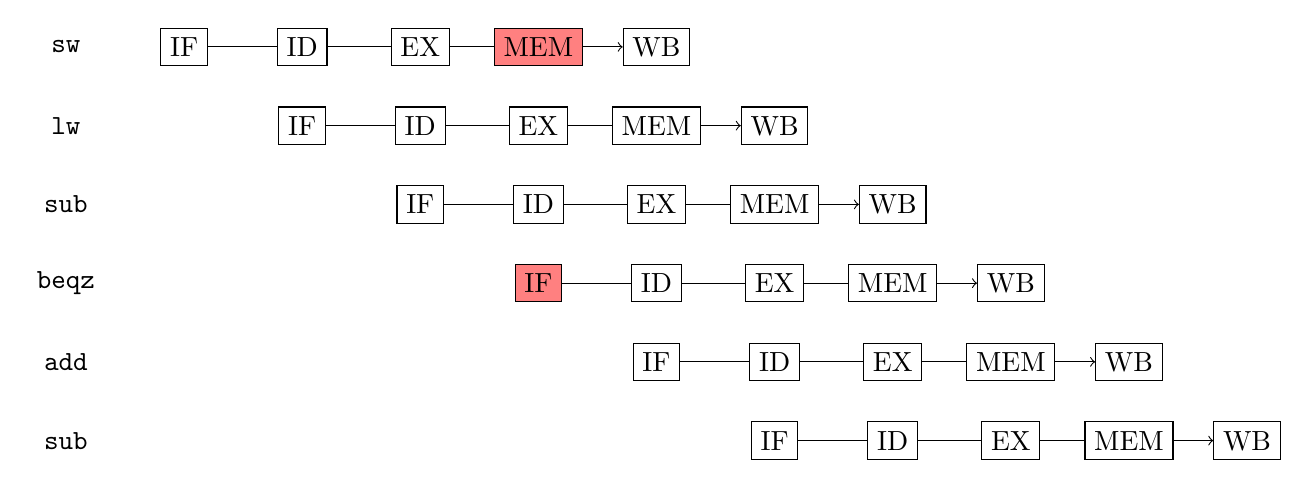
\begin{tikzpicture}
		\draw 
		(-1.5, 0) node {\texttt{sw}}
		(0, 0) node [rectangle, draw] (IF1) {IF}
		(1.5, 0) node [rectangle, draw] (ID1) {ID}
		(3, 0) node [rectangle, draw] (EX1) {EX}
		(4.5, 0) node [rectangle, draw, fill=red!50] (MEM1) {MEM}
		(6, 0) node [rectangle, draw] (WB1) {WB};
		\draw[->] (IF1) -- (ID1) -- (EX1) -- (MEM1) -- (WB1);

		\draw 
		(-1.5, -1) node {\texttt{lw}}
		(1.5, -1) node [rectangle, draw] (IF2) {IF}
		(3, -1) node [rectangle, draw] (ID2) {ID}
		(4.5, -1) node [rectangle, draw] (EX2) {EX}
		(6, -1) node [rectangle, draw] (MEM2) {MEM}
		(7.5, -1) node [rectangle, draw] (WB2) {WB};
		\draw[->] (IF2) -- (ID2) -- (EX2) -- (MEM2) -- (WB2);
		
		\draw 
		(-1.5, -2) node {\texttt{sub}}
		(3, -2) node [rectangle, draw] (IF3) {IF}
		(4.5, -2) node [rectangle, draw] (ID3) {ID}
		(6, -2) node [rectangle, draw] (EX3) {EX}
		(7.5, -2) node [rectangle, draw] (MEM3) {MEM}
		(9, -2) node [rectangle, draw] (WB3) {WB};
		\draw[->] (IF3) -- (ID3) -- (EX3) -- (MEM3) -- (WB3);

		\draw 
		(-1.5, -3) node {\texttt{beqz}}
		(4.5, -3) node [rectangle, draw, fill=red!50] (IF4) {IF}
		(6, -3) node [rectangle, draw] (ID4) {ID}
		(7.5, -3) node [rectangle, draw] (EX4) {EX}
		(9, -3) node [rectangle, draw] (MEM4) {MEM}
		(10.5, -3) node [rectangle, draw] (WB4) {WB};
		\draw[->] (IF4) -- (ID4) -- (EX4) -- (MEM4) -- (WB4);

		\draw 
		(-1.5, -4) node {\texttt{add}}
		(6, -4) node [rectangle, draw] (IF5) {IF}
		(7.5, -4) node [rectangle, draw] (ID5) {ID}
		(9, -4) node [rectangle, draw] (EX5) {EX}
		(10.5, -4) node [rectangle, draw] (MEM5) {MEM}
		(12, -4) node [rectangle, draw] (WB5) {WB};
		\draw[->] (IF5) -- (ID5) -- (EX5) -- (MEM5) -- (WB5);

		\draw 
		(-1.5, -5) node {\texttt{sub}}
		(7.5, -5) node [rectangle, draw] (IF6) {IF}
		(9, -5) node [rectangle, draw] (ID6) {ID}
		(10.5, -5) node [rectangle, draw] (EX6) {EX}
		(12, -5) node [rectangle, draw] (MEM6) {MEM}
		(13.5, -5) node [rectangle, draw] (WB6) {WB};
		\draw[->] (IF6) -- (ID6) -- (EX6) -- (MEM6) -- (WB6);
	\end{tikzpicture}
\end{center}

Hence, we stall the \texttt{beqz} instruction for one cycle.
But the hazard still exists.
\begin{center}
	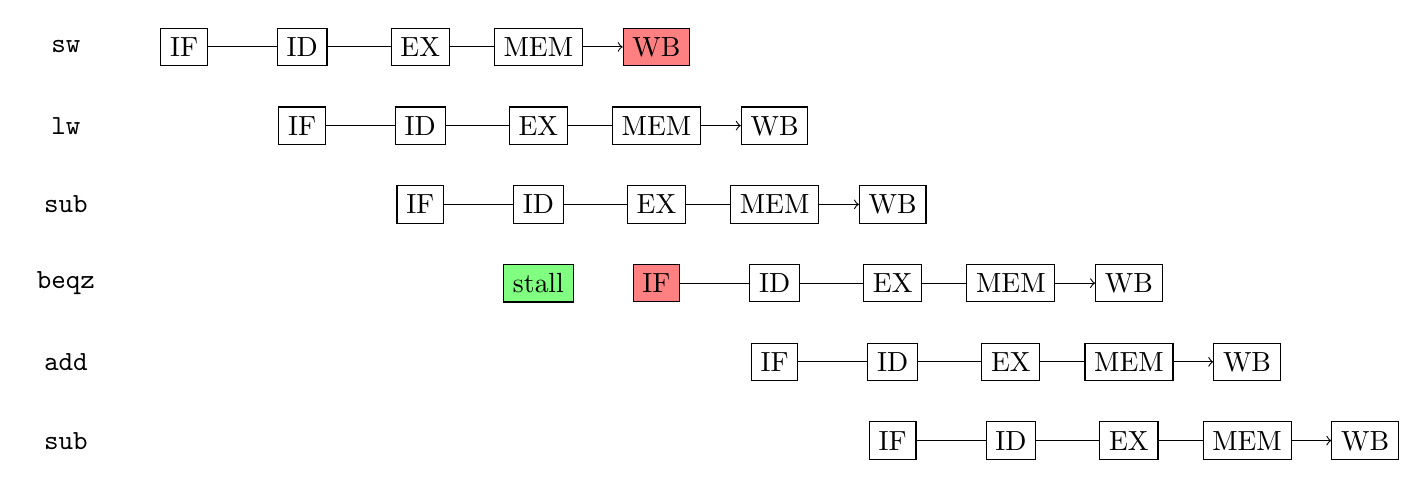
\begin{tikzpicture}
		\draw 
		(-1.5, 0) node {\texttt{sw}}
		(0, 0) node [rectangle, draw] (IF1) {IF}
		(1.5, 0) node [rectangle, draw] (ID1) {ID}
		(3, 0) node [rectangle, draw] (EX1) {EX}
		(4.5, 0) node [rectangle, draw] (MEM1) {MEM}
		(6, 0) node [rectangle, draw, fill=red!50] (WB1) {WB};
		\draw[->] (IF1) -- (ID1) -- (EX1) -- (MEM1) -- (WB1);

		\draw 
		(-1.5, -1) node {\texttt{lw}}
		(1.5, -1) node [rectangle, draw] (IF2) {IF}
		(3, -1) node [rectangle, draw] (ID2) {ID}
		(4.5, -1) node [rectangle, draw] (EX2) {EX}
		(6, -1) node [rectangle, draw] (MEM2) {MEM}
		(7.5, -1) node [rectangle, draw] (WB2) {WB};
		\draw[->] (IF2) -- (ID2) -- (EX2) -- (MEM2) -- (WB2);
		
		\draw 
		(-1.5, -2) node {\texttt{sub}}
		(3, -2) node [rectangle, draw] (IF3) {IF}
		(4.5, -2) node [rectangle, draw] (ID3) {ID}
		(6, -2) node [rectangle, draw] (EX3) {EX}
		(7.5, -2) node [rectangle, draw] (MEM3) {MEM}
		(9, -2) node [rectangle, draw] (WB3) {WB};
		\draw[->] (IF3) -- (ID3) -- (EX3) -- (MEM3) -- (WB3);

		\draw 
		(-1.5, -3) node {\texttt{beqz}}
		(4.5, -3) node [rectangle, draw, fill=green!50] (stall) {stall}
		(6, -3) node [rectangle, draw, fill=red!50] (IF4) {IF}
		(7.5, -3) node [rectangle, draw] (ID4) {ID}
		(9, -3) node [rectangle, draw] (EX4) {EX}
		(10.5, -3) node [rectangle, draw] (MEM4) {MEM}
		(12, -3) node [rectangle, draw] (WB4) {WB};
		\draw[->] (IF4) -- (ID4) -- (EX4) -- (MEM4) -- (WB4);

		\draw 
		(-1.5, -4) node {\texttt{add}}
		(7.5, -4) node [rectangle, draw] (IF5) {IF}
		(9, -4) node [rectangle, draw] (ID5) {ID}
		(10.5, -4) node [rectangle, draw] (EX5) {EX}
		(12, -4) node [rectangle, draw] (MEM5) {MEM}
		(13.5, -4) node [rectangle, draw] (WB5) {WB};
		\draw[->] (IF5) -- (ID5) -- (EX5) -- (MEM5) -- (WB5);

		\draw 
		(-1.5, -5) node {\texttt{sub}}
		(9, -5) node [rectangle, draw] (IF6) {IF}
		(10.5, -5) node [rectangle, draw] (ID6) {ID}
		(12, -5) node [rectangle, draw] (EX6) {EX}
		(13.5, -5) node [rectangle, draw] (MEM6) {MEM}
		(15, -5) node [rectangle, draw] (WB6) {WB};
		\draw[->] (IF6) -- (ID6) -- (EX6) -- (MEM6) -- (WB6);
	\end{tikzpicture}
\end{center}

Hence, we stall the \texttt{beqz} instruction for one more cycle.
The hazard is resolved.

\begin{center}
	\resizebox{\linewidth}{!}{
	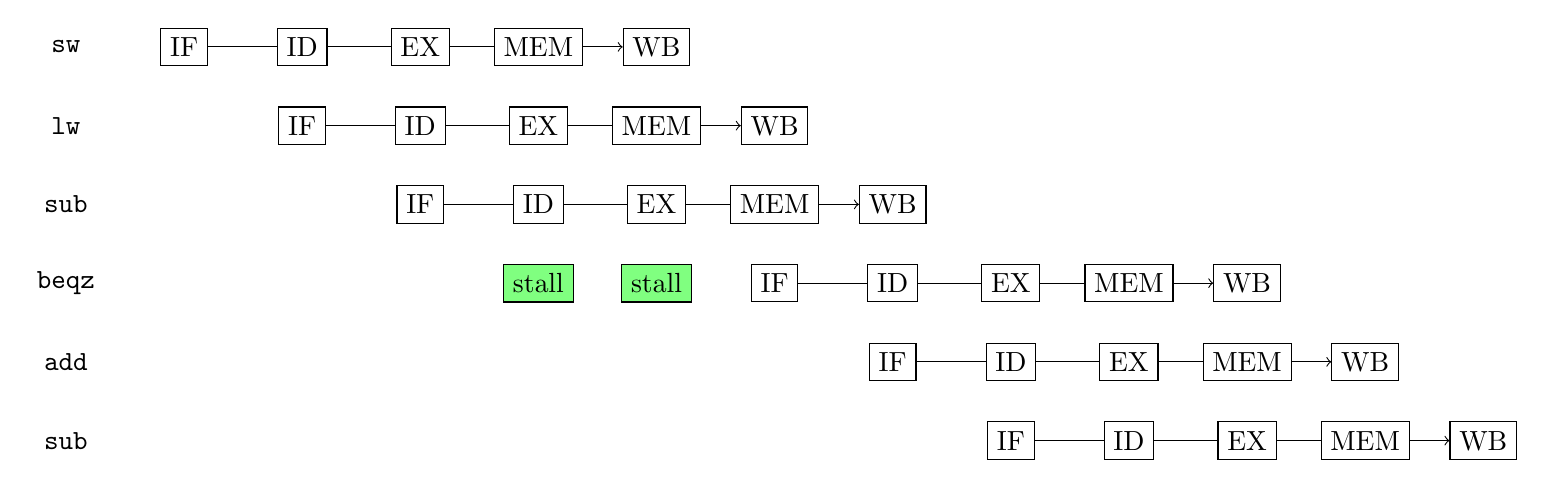
\begin{tikzpicture}
		\draw 
		(-1.5, 0) node {\texttt{sw}}
		(0, 0) node [rectangle, draw] (IF1) {IF}
		(1.5, 0) node [rectangle, draw] (ID1) {ID}
		(3, 0) node [rectangle, draw] (EX1) {EX}
		(4.5, 0) node [rectangle, draw] (MEM1) {MEM}
		(6, 0) node [rectangle, draw] (WB1) {WB};
		\draw[->] (IF1) -- (ID1) -- (EX1) -- (MEM1) -- (WB1);

		\draw 
		(-1.5, -1) node {\texttt{lw}}
		(1.5, -1) node [rectangle, draw] (IF2) {IF}
		(3, -1) node [rectangle, draw] (ID2) {ID}
		(4.5, -1) node [rectangle, draw] (EX2) {EX}
		(6, -1) node [rectangle, draw] (MEM2) {MEM}
		(7.5, -1) node [rectangle, draw] (WB2) {WB};
		\draw[->] (IF2) -- (ID2) -- (EX2) -- (MEM2) -- (WB2);
		
		\draw 
		(-1.5, -2) node {\texttt{sub}}
		(3, -2) node [rectangle, draw] (IF3) {IF}
		(4.5, -2) node [rectangle, draw] (ID3) {ID}
		(6, -2) node [rectangle, draw] (EX3) {EX}
		(7.5, -2) node [rectangle, draw] (MEM3) {MEM}
		(9, -2) node [rectangle, draw] (WB3) {WB};
		\draw[->] (IF3) -- (ID3) -- (EX3) -- (MEM3) -- (WB3);

		\draw 
		(-1.5, -3) node {\texttt{beqz}}
		(4.5, -3) node [rectangle, draw, fill=green!50] (stall) {stall}
		(6, -3) node [rectangle, draw, fill=green!50] (stall) {stall}
		(7.5, -3) node [rectangle, draw] (IF4) {IF}
		(9, -3) node [rectangle, draw] (ID4) {ID}
		(10.5, -3) node [rectangle, draw] (EX4) {EX}
		(12, -3) node [rectangle, draw] (MEM4) {MEM}
		(13.5, -3) node [rectangle, draw] (WB4) {WB};
		\draw[->] (IF4) -- (ID4) -- (EX4) -- (MEM4) -- (WB4);

		\draw 
		(-1.5, -4) node {\texttt{add}}
		(9, -4) node [rectangle, draw] (IF5) {IF}
		(10.5, -4) node [rectangle, draw] (ID5) {ID}
		(12, -4) node [rectangle, draw] (EX5) {EX}
		(13.5, -4) node [rectangle, draw] (MEM5) {MEM}
		(15, -4) node [rectangle, draw] (WB5) {WB};
		\draw[->] (IF5) -- (ID5) -- (EX5) -- (MEM5) -- (WB5);

		\draw 
		(-1.5, -5) node {\texttt{sub}}
		(10.5, -5) node [rectangle, draw] (IF6) {IF}
		(12, -5) node [rectangle, draw] (ID6) {ID}
		(13.5, -5) node [rectangle, draw] (EX6) {EX}
		(15, -5) node [rectangle, draw] (MEM6) {MEM}
		(16.5, -5) node [rectangle, draw] (WB6) {WB};
		\draw[->] (IF6) -- (ID6) -- (EX6) -- (MEM6) -- (WB6);
	\end{tikzpicture}
	}
\end{center}

Although at some points we seem to be executing the \texttt{WB} and \texttt{IF} stages simultaneously, but the instruction does not actually write back to memory and the \texttt{WB} stage is just for pipelining (For example, the \texttt{WB} stage of the \texttt{lw} overlaps with the \texttt{IF} stage of the \texttt{beqz} instruction, but the \texttt{lw} instruction does not write back to memory).

\subsection*{b)}

No, we add proper hardware to solve structural hazards, not by reordering instructions.

\subsection*{c)}

The \texttt{NOP} instruction is itself an instruction, and needs to be fetched in the \texttt{IF} stage.
Hence, it will not resolve this structural hazard caused by \texttt{IF} stage overlaps with other memory stages.

\section*{Problem 4}

\subsection*{a)}

\begin{center}
	\begin{tabular}{|l|l|}
		\hline
		Memory & ALU/Branch \\ \hline
		& \texttt{li x12, 0} \\ \hline
		& \texttt{jal ENT} \\ \hline
		& \texttt{bne x12, x13, TOP} \\ \hline
		& \texttt{slli x5, x12, 2} \\ \hline
		& \texttt{add x6, x10, x5} \\ \hline
		\texttt{lw x7, 0(x6)} & \\ \hline
		\texttt{lw x29, 4(x6)} & \\ \hline
		& \texttt{sub x30, x7, x29} \\ \hline
		& \texttt{add x31, x11, x5} \\ \hline
		\texttt{sw x30, 0(x31)} & \texttt{addi x12, x12, 2} \\ \hline
		& \texttt{bne x12, x13, TOP} \\ \hline
		& \texttt{slli x5, x12, 2} \\ \hline
		& \texttt{add x6, x10, x5} \\ \hline
		\texttt{lw x7, 0(x6)} & \\ \hline
		\texttt{lw x29, 4(x6)} & \\ \hline
		& \texttt{sub x30, x7, x29} \\ \hline
		& \texttt{add x31, x11, x5} \\ \hline
		\texttt{sw x30, 0(x31)} & \texttt{addi x12, x12, 2} \\ \hline
		& \texttt{bne x12, x13, TOP} \\ \hline
	\end{tabular}
\end{center}

\subsection*{b)}

For each iteration, we need to run every line from label \texttt{TOP} to label \texttt{ENT}.

Assume the time cost for each instruction is 1 cycle.
And we consider the stall caused by load-use hazard.
For a one-issue processor, one iteration will take 10 cycles.
For a two-issue processor, one iteration will take 9 cycles.

Hence, the speedup ratio will be $\frac{10}{9} = 1.111$.

\subsection*{c)}

An optimized version of the code for one-issue processor is shown below:
\begin{minted}{asm}
	slli x5, x13, 2
	add x6, x10, x5
	add x7, x11, x5
	Loop: 
	beqz x5, Exit
	lw x29, 0(x6)
	lw x30, 4(x6)
	addi x5, x5, -8
	sub x31, x29, x30
	sw x31, 0(x7)
	addi x6, x6, -8
	addi x7, x7, -8
	j Loop
	Exit:
\end{minted}

\subsection*{d)}

An optimized version of the code for two-issue processor is shown below:

\begin{center}
	\begin{tabular}{|l|l|}
		\hline
		Memory & ALU/Branch \\ \hline
		\texttt{lw x29, 0(x6)} & \texttt{beqz x5, Exit} \\ \hline
		\texttt{lw x30, 4(x6)} & \texttt{addi x5, x5, -8} \\ \hline
		& \texttt{sub x31, x29, x30} \\ \hline
		\texttt{sw x31, 0(x7)} & \texttt{addi x6, x6, -8} \\ \hline
		& \texttt{addi x7, x7, -8} \\ \hline
		& \texttt{j Loop} \\ \hline
	\end{tabular}
\end{center}

\subsection*{e)}

The speed up ratio will be $\frac{9}{6} = 1.5$.

\end{document}